\documentclass[12pt]{article}%
\usepackage{amsfonts}
\usepackage{fancyhdr}
\usepackage{comment}
\usepackage[a4paper, top=2.5cm, bottom=2.5cm, left=2.2cm, right=2.2cm]%
{geometry}
\usepackage{times}
\usepackage{amsmath, nccmath}
\usepackage{changepage}
\usepackage{amssymb}
\usepackage{graphicx}%
\usepackage{lipsum}
\usepackage{array}
\usepackage{listings}
\usepackage{color}
\usepackage{xcolor}

\delimitershortfall-1sp
\newcommand\abs[1]{\left|#1\right|}
\graphicspath{ {./images/} }

\DeclareUnicodeCharacter{2212}{-}
\definecolor{lightgray}{RGB}{214, 219, 223}
\definecolor{limegreen}{RGB}{11, 83, 69}
\definecolor{blue}{RGB}{0, 70, 255}
\lstdefinestyle{mystyle}{
    backgroundcolor=\color{lightgray},   
    commentstyle=\color{limegreen},
    keywordstyle=\color{blue}
}
 
\lstset{style=mystyle}
\makeatletter
\renewcommand{\maketitle}{\bgroup\setlength{\parindent}{0pt}
\begin{flushleft}
  \textbf{\@title}

  \@author
  \@date
\end{flushleft}\egroup
}
\makeatother


\begin{document}

\title{Weekly Assignment 4}
\author{Leong Kai Ler \\ 15334636 \\   }
\date{February 16, 2019}
\maketitle

\section*{Question 1}
Consider an experiment where we roll two 6-sided dice. Let random variable Y be the sum of the values rolled. The sample space is $\{(1, 1), (1, 2), (1, 3), . . . , (6, 6)\}$ and recall that a random event is a subset of the sample space.
\subsection*{Problem part a}
What random event corresponds to $Y = 2$ ?
\subsection*{Solution part a}
Minimum value each dice can produce is 1, so to get a sum of 2, both dice rolled can only produce 1 and not higher. Hence, \\
\begin{equation*}
Y = \{(1,1)\}
\end{equation*}
\subsection*{Problem part b}
What event corresponds to $Y = 3$ ?
\subsection*{Solution part b}
To get a sum of 3, one dice have to produce 1 while the other produce 2. Hence \\ 
\begin{equation*}
Y = \{(1,2), (2,1)\}
\end{equation*}
\subsection*{Problem part c}
What event corresponds to $Y = 4$ ?
\subsection*{Solution part c}
To get a sum of 4, consider the following cases:
\begin{itemize}
\item First dice rolled produce 1: \\
Then, second dice rolled must produce 3.
\item First dice rolled produce 2: \\
Then, second dice rolled must produce 2.
\item First dice rolled produce 3: \\
Then, second dice rolled must produce 1.
\end{itemize}
So, \\
\begin{equation*}
Y = \{(1,3), (2,2), (3,1)\}
\end{equation*}
\subsection*{Problem part d}
Now let $X$ be the indicator random variable associated with the event $\{(1, 1), (2, 2), (3, 3)\}$. \\
What is the probabilities that $X = 1$ ?
\subsection*{Solution part d}
\begin{eqnarray*}
P(X) & = & \frac{\abs{X}}{\abs{S}} \\
 	 & = & \frac{3}{6^2} \\
 	 & = & \frac{1}{12} \\
 	 & \approx & 0.0833
\end{eqnarray*}
\newpage
\section*{Question 2}
Let $X$ represent the difference between the number of heads and the number of tails obtained when a coin is tossed 3 times.
\subsection*{Problem part a}
What are the possible values of $X$ ?
\subsection*{Solution part a}
Consider the following possible cases:
\begin{itemize}
\item Getting 3 Heads and 0 tails: \\
Difference is 3
\item Getting 2 Heads and 1 tails: \\
Difference is 1
\item Getting 1 Heads and 2 tails: \\
Difference is -1
\item Getting 0 Heads and 3 tails: \\
Difference is -3
\end{itemize} 
So, the possible values of $X$ are $\{-3,-1,1,3\}$.
\subsection*{Problem part b}
What is $P(X = −3)$ ?
\subsection*{Solution part b}
Since a coin has two sides and tossing three times will give $2^3=8$ possible sequence results, hence $\abs{S} = 8$. $P(X = −3) = $ Probability of getting $\{T,T,T\}$ OR 3 Tails. So,
\begin{eqnarray*}
P(X = −3) & = & \frac{\abs{(X =-3)}}{\abs{S}}\\
		  & = & \frac{1}{8} \\
		  & = & 0.1250
\end{eqnarray*}
\subsection*{Problem part c}
What is $P(X = −1)$ ?
\subsection*{Solution part c}
$P(X = −1) = $ Probability of getting 2 Tails,i.e $\{(T,T,H),(T,H,T),(H,T,T)\}$. So,
\begin{eqnarray*}
P(X = −1) & = & \frac{\abs{(X =-1)}}{\abs{S}}\\
		  & = & \frac{3}{8} \\
		  & = & 0.3750
\end{eqnarray*}
\subsection*{Problem part d}
If the coin is assumed fair, calculate the PMF and CDF of X and plot a sketch of both.
\subsection*{Solution part d}
Variable $X$ takes values in $\{-3,-1,1,3\}$. To calculate its CDF, we can compute the respective PMF first:
\begin{itemize}
\item $P(X=-3)=\frac{1}{8}$
\item $P(X=-1)=\frac{3}{8}$
\item $P(X=1)=\frac{3}{8}$
\item $P(X=3)=\frac{1}{8}$
\end{itemize}

\subsubsection*{PMF diagram:}
\begin{center}
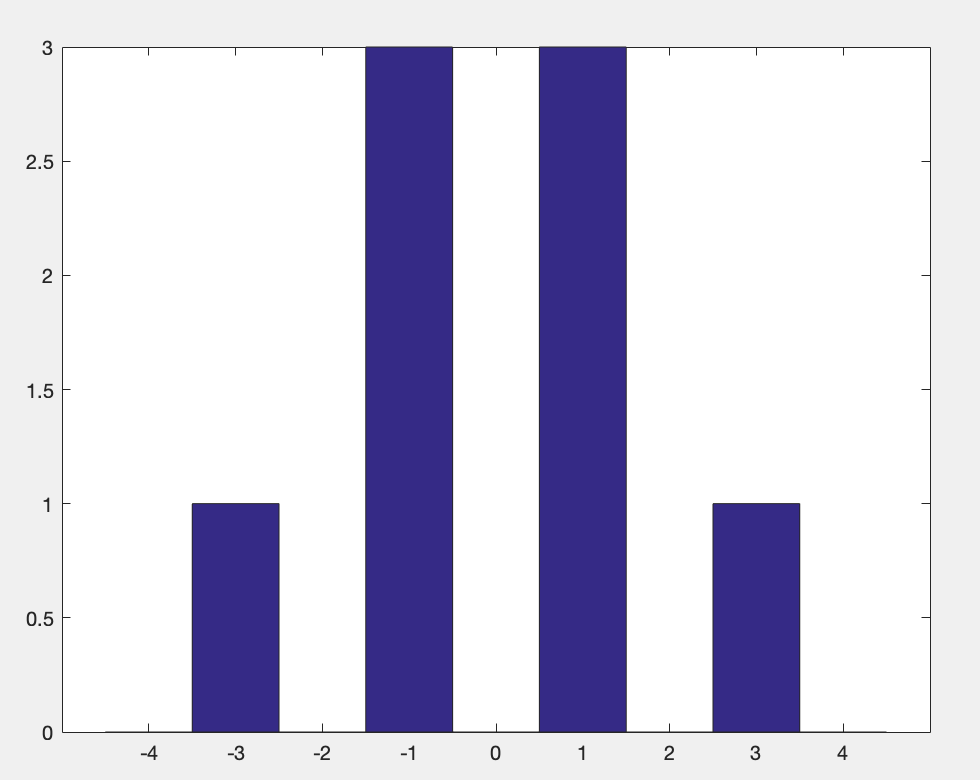
\includegraphics[scale=0.8]{pmf} \\
\end{center}

The random variable $X$ has a CDF of:
\[ P(X) =
  \begin{cases}
    0.125       	  & \quad x = -3 \\
    0.5  	    	  & \quad x = -1 \\
  	0.875  	    	  & \quad x = 1 \\
    1       		  & \quad x = 3 
  \end{cases}
\]

\subsubsection*{CDF diagram:}
\begin{center}
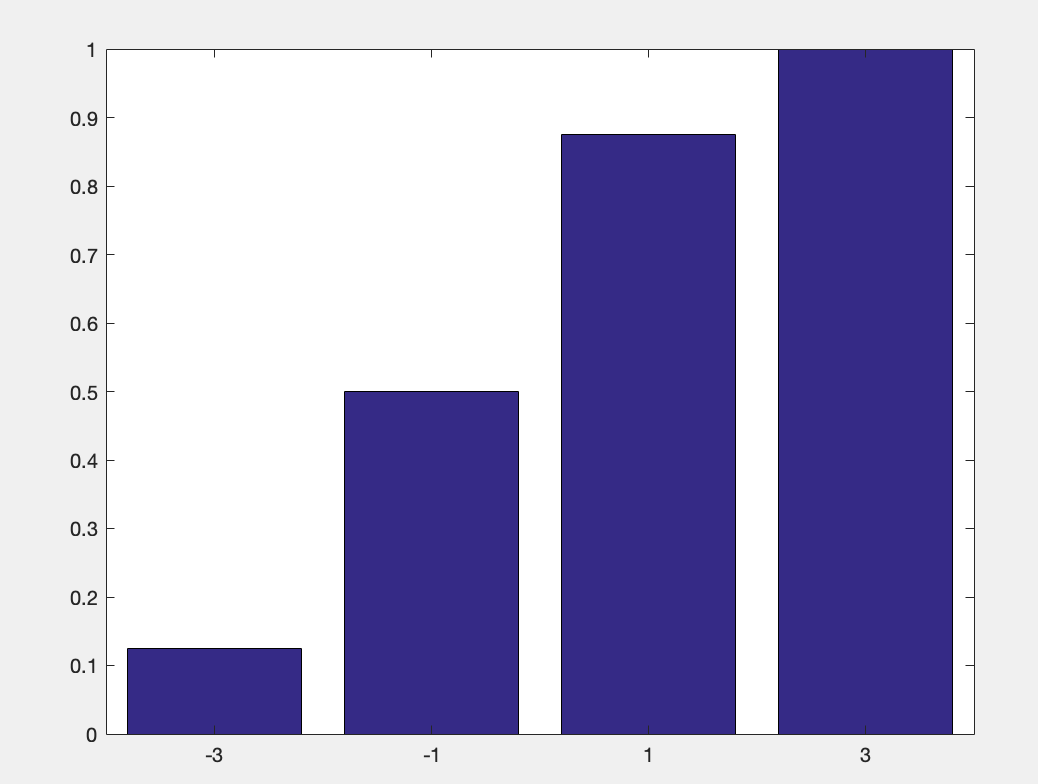
\includegraphics[scale=0.8]{cdf} \\
\end{center}
\newpage
\section*{Question 3}
Four 6-sided dice are rolled. The dice are fair, so each one has equal probability of producing a value in $\{1,2,3,4,5,6\}$. Let X =the minimum of the four values rolled. (It is fine if more than one of the dice has the minimal value.)
\subsection*{Problem part a}
What is $P(X \geq 1)$ ?
\subsection*{Solution part a}
Since the minimum value on a dice is 1, it doesn't matter how it is rolled, the result will always be more or equal than 1. Hence, 
\begin{eqnarray*}
P(X \geq 1) & = & \frac{6^4}{6^4} \\
			& = & 1
\end{eqnarray*}
\subsection*{Problem part b}
What is P $(X \geq 2)$ ?
\subsection*{Solution part b}
For every dice roll, there is a $\frac{5}{6}$ chance of getting values higher than 1, namely 2 to 6. Hence, rolling 4 dice will have a probability of: 
\begin{eqnarray*}
P(X \geq 1) & = & (\frac{5}{6})^4 \\
			& = & \frac{625}{1296} \\
			& \approx & 0.4823
\end{eqnarray*}
\subsection*{Problem part c}
What is the CDF of $X$ i.e. $P(X \leq k)$ for all values of $k$ ?
\subsection*{Solution part c}
To calculate the CDF for each $P(X \leq k)$ for each $k$, we can just reverse subtract 1 by the probability of not getting any values equal or less than k. \\

Let $R$ be the event of not rolling values $\leq k$.
\begin{fleqn}[\parindent]
\begin{equation*}
\begin{split}
P(X\leq1) = & 1 - P(R) \\
		  = & 1 - (\frac{5}{6})^4 \\
		  = & 1 - \frac{625}{1296} \\
		  = & \frac{671}{1296} \\
P(X\leq2) = & 1 - P(R) \\
		  = & 1 - (\frac{4}{6})^4 \\
		  = & 1 - \frac{16}{81} \\
		  = & \frac{65}{81} \\
P(X\leq3) = & 1 - P(R) \\
		  = & 1 - (\frac{3}{6})^4 \\
		  = & 1 - \frac{1}{16} \\
		  = & \frac{15}{16} \\
P(X\leq4) = & 1 - P(R) \\
		  = & 1 - (\frac{2}{6})^4 \\
		  = & 1 - \frac{1}{81} \\
		  = & \frac{80}{81} \\
P(X\leq5) = & 1 - P(R) \\
		  = & 1 - (\frac{1}{6})^4 \\
		  = & 1 - \frac{1}{1296} \\
		  = & \frac{1295}{1296} \\
P(X\leq6) = & 1 - P(R) \\
		  = & 1 - (\frac{0}{6})^4 \\
		  = & 1 - 0 \\
		  = & 1 \\
\end{split}
\end{equation*}
\end{fleqn}



\[ P(X) =
  \begin{cases}
    \frac{671}{1296}     & \quad 1 \leq x < 2 \\
    \frac{65}{81} 	  	  & \quad 2 \leq x < 3 \\
  	\frac{15}{16}  	  	  & \quad 3 \leq x < 4 \\
    \frac{80}{81}     & \quad 4 \leq x < 5 \\
    \frac{1295}{1296}     & \quad 5 \leq x < 6 \\
    1     & \quad 6 \leq x 
  \end{cases}
\]
\end{document}